\chapter{Scripts and Functions}

\section{Script files}
A \textit{script} file is a text file that contains a series of \mlab commands that you would type at the command prompt. A \textit{script} file is one type of m-file (\textit{.m} file extension), the other type being a \textit{function} file which will be examined in Section~\ref{sec:functions}. Script files are useful when you have to repeat a set of commands, often only changing the value of one variable every time. By writing a script file you are saving your work for later use. Script files work on variables in the current workspace, and results obtained from running a script are left in the current workspace.

New script files can be created by clicking on the \textit{New M-File} icon in the \mlab Window toolbar, shown in Figure~\ref{fig:new_script}. This launches the \mlab Editor with a blank M-File.
\begin{figure}[h]
	\myfloatalign
	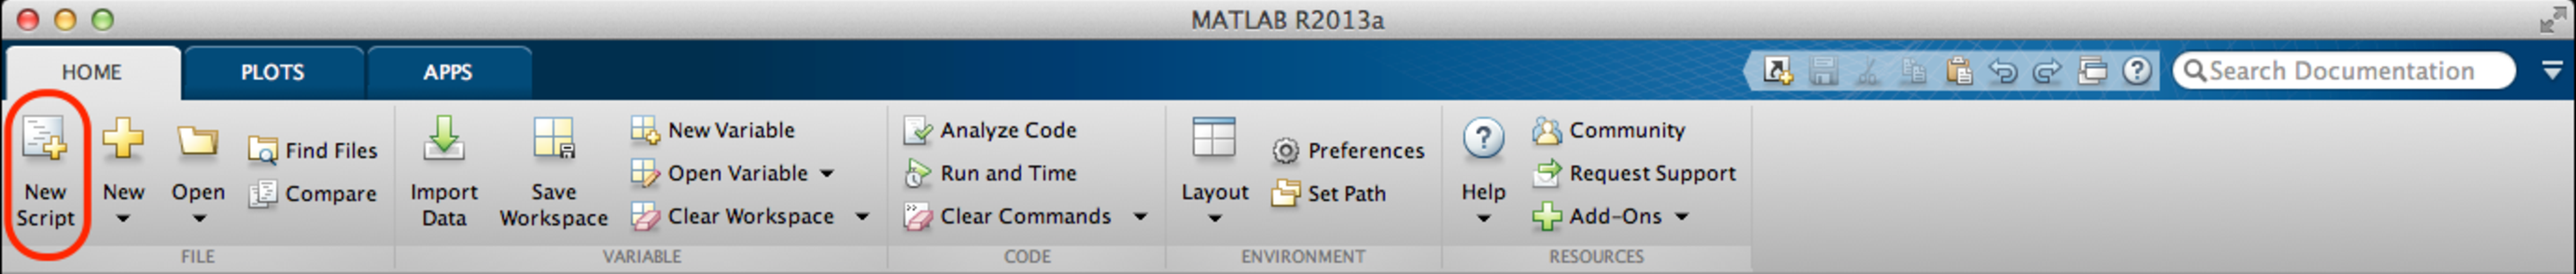
\includegraphics[width=0.9\linewidth]{Graphics/Unit03/new_script}
	\caption{\textit{New M-File} toolbar icon in \mlab Window}
	\label{fig:new_script}
\end{figure}

Listing~\ref{lst:my_surf} presents the commands from Listing~\ref{lst:surf} in the form of a script file. The script file has been saved as \textit{my\_surf.m}, and can be run by either typing \mcode{my_surf} at the command prompt, or clicking the \textit{Save and run} icon in the Editor Window toolbar, as shown in Figure~\ref{fig:run_script}. Copy and paste the example into a new script file, and run it to see the results for yourself.
\begin{figure}[h]
	\myfloatalign
	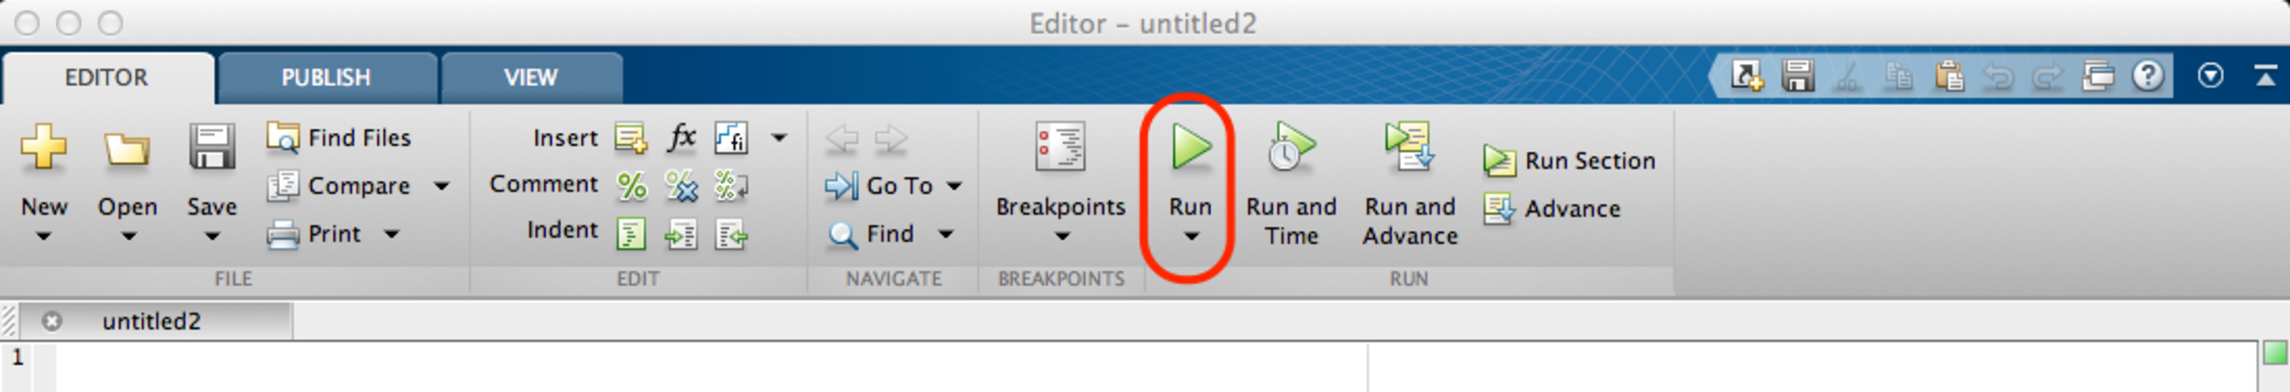
\includegraphics[width=0.9\linewidth]{Graphics/Unit03/run_script}
	\caption{\textit{Save and run} toolbar icon in Editor Window}
	\label{fig:run_script}
\end{figure}

\newpage
\lstinputlisting[caption={\textit{my\_surf.m} - Script to plot a surface},label=lst:my_surf]{MATLAB-code/Document/my_surf.m}

\subsubsection{Comments:}
\begin{itemize}
\item It is extremely useful, for both yourself and others, to put comments in your script files. A comment is always preceded with a percent sign (\mcode{\%}) which tells \mlab not to execute the rest of the line as a command.
\item Script file names MUST NOT contain spaces (replace a space with the underscore), start with a number, be names of built-in functions, or be variable names.
\item It is a good idea to use the \mcode{clear all} and \mcode{clc} commands as the first commands in your script to clear any existing variables from the \mlab workspace and clear up the Command Window before you begin.
\end{itemize}

\addtolength{\parindent}{-4mm}
\fcolorbox{myborderblue}{myblue}{%
\begin{minipage}{\linewidth}
\begin{minipage}{6mm}

\includegraphics[scale=0.03]{Graphics/General/help_icon}
\end{minipage}
\textit{Writing good scripts} \\
Here are some useful tips that you should follow to make your script files easy to follow and easy to understand by others, or even yourself after a few weeks!\footnote{Adapted from \citet{Patzer:2003fk}.}
\begin{itemize}
\item Script files should have a header section that identifies:
	\begin{itemize}
	\item What the program does
	\item Who the author is
	\item When the program was written or last revised
	\item The variable dictionary \ie\ a list of all variables their meanings and units
	\end{itemize}
\item Use plenty of white space to make your program easy to read.
\item Use plenty of comments! In particular define all variables and their units in the variable dictionary.
\item Use meaningful names for variables. Don't be afraid of being verbose \eg\ use \mcode{steel_area} in preference to \mcode{sa}.
\item Remember to use the \mcode{clear all} and \mcode{clc} commands at the start of your script.
\end{itemize}
\end{minipage}%
}\\
\addtolength{\parindent}{4mm}
\vspace{5mm}

%%%%%%%%%%%%%%%%%%%%%%%%%%%%%%%%%%%%%%%%%%%%%%
% Screencast: Creating a simple script
%%%%%%%%%%%%%%%%%%%%%%%%%%%%%%%%%%%%%%%%%%%%%%
\addtolength{\parindent}{-4mm}
\fcolorbox{myborderblue}{myblue}{%
\begin{minipage}{\linewidth}
\begin{minipage}{6mm}

\includegraphics[scale=0.03]{Graphics/General/screencast_icon}
\end{minipage}
\href{http://www.eng.ed.ac.uk/teaching/courses/matlab/unit03/simple-script.shtml}{\screencast{Creating a simple script}}\\
(http://www.eng.ed.ac.uk/teaching/courses/matlab/unit03/simple-script.shtml)
\end{minipage}%
}\\
\addtolength{\parindent}{4mm}
\vspace{5mm}

\addtolength{\parindent}{-4mm}
\fcolorbox{myborderblue}{myblue}{%
\begin{minipage}{\linewidth}
\begin{minipage}{6mm}

\includegraphics[scale=0.03]{Graphics/General/help_icon}
\end{minipage}
\textit{The \mcode{input} function} \\
The \mcode{input} function is used to request user input and assign it to a variable. For example \mcode{x = input('Enter a number: ');} will display the text \mcode{Enter a number: } in the Command Window and then wait until the user enters something. Whatever is entered will be assigned to the variable \mcode{x}.
\end{minipage}%
}\\
\addtolength{\parindent}{4mm}
\vspace{5mm}

\addtolength{\parindent}{-4mm}
\fcolorbox{myborderblue}{myblue}{%
\begin{minipage}{\linewidth}
\begin{minipage}{6mm}

\includegraphics[scale=0.03]{Graphics/General/help_icon}
\end{minipage}
\textit{The \mcode{disp} function} \\
The \mcode{disp} function can be used display strings of text to the Command Window \eg\ \mcode{disp('I am a string of text')}. You can also display numbers by converting them to strings \eg\ \mcode{disp(num2str(10))}. The \mcode{num2str} function simply converts the number 10 to a string that can be displayed by the \mcode{disp} function. You can also combine the display of text and numbers \eg\ \mcode{disp(['Factorial '} \mcode{num2str(x) ' is '} \mcode{num2str(y)])}. Notice the use of spaces to denote the separate elements of the string, and square brackets around the string to concatenate it together.
\end{minipage}%
}\\
\addtolength{\parindent}{4mm}

%%%%%%%%%%%%%%%%%%%%%%%%%%%%%%%%%%%%%%%%%%%%%%
% Exercise 5: Scripts
%%%%%%%%%%%%%%%%%%%%%%%%%%%%%%%%%%%%%%%%%%%%%%
\addtolength{\parindent}{-4mm}
\fcolorbox{myborderblue}{myblue}{%
\begin{minipage}{\linewidth}
\begin{minipage}{6mm}

\includegraphics[scale=0.035]{Graphics/General/exercise_icon}
\end{minipage}
\exercise{\textit{Exercise 5: Scripts}} \\
Write your own script files to solve the following problems:
\begin{enumerate}
\item The absolute pressure at the bottom of a liquid store tank that is vented to the atmosphere is given by:
\begin{equation*}
P_{\textrm{abs,bottom}} = \rho g h + P_{\textrm{outside}},
\end{equation*}
where:
\begin{align*}
P_{\textrm{abs,bottom}} &= \textrm{the absolute pressure at the bottom of the storage tank ($Pa$)} \\
\rho &= \textrm{liquid density ($kg/m^3$)} \\
g &= \textrm{acceleration due to gravity ($m/s^2$)} \\
h &= \textrm{height of the liquid ($m$)} \\
P_{\textrm{outside}} &= \textrm{outside atmospheric pressure ($Pa$)}
\end{align*}
Find $P_{\textrm{abs,bottom}}$ in SI units if $\rho=1000~kg/m^3$, $g=32.2~ft/s^2$, $h=7~yd$, and $P_{\textrm{outside}}=1~atm$. \\
Here are some tips to help you get started:
	\begin{itemize}
	\item Remember your header section and variable dictionary.
	\item Use \mcode{input} functions to gather information from the user.
	\item Convert all units to SI before performing the calculation. Use the following conversion factors:
		\renewcommand{\labelitemii}{}
		\begin{itemize}
		\item \mcode{ft_to_m = 0.3048}
		\item \mcode{yd_to_m = 0.9144}
		\item \mcode{atm_to_Pa = 1.013E5}
		\end{itemize}
	\item Calculate $P_{\textrm{abs,bottom}}$
	\end{itemize}
\footnotesize{\textit{[Answers: $164121~Pa$]}\\
Example adapted from \citet{Patzer:2003fk}}	
\normalsize
\end{enumerate}
\end{minipage}%
}\\
\addtolength{\parindent}{4mm}

%%%%%%%%%%%%%%%%%%%%%%%%%%%%%%%%%%%%%%%%%%%%%%
% Exercise 5: Scripts (continued)
%%%%%%%%%%%%%%%%%%%%%%%%%%%%%%%%%%%%%%%%%%%%%%
\addtolength{\parindent}{-4mm}
\fcolorbox{myborderblue}{myblue}{%
\begin{minipage}{\linewidth}
\begin{minipage}{6mm}

\includegraphics[scale=0.035]{Graphics/General/exercise_icon}
\end{minipage}
\textit{Exercise 5: Scripts (continued)}
\begin{enumerate}
\setcounter{enumi}{1}
\item A pipeline at an oil refinery is carrying oil to a large storage tank. The pipe has a 20~inch internal diameter. The oil is flowing at 5~$ft/s$ and its density is 57~$lb/ft^3$. What is the mass flow rate of oil in SI units? What is the mass and volume of oil, in SI units, that flows in a 24~hour period? The flow rate of oil is given by:
\begin{equation*}
\dot{M} = \rho \nu A,
\end{equation*}
where:
\begin{align*}
\dot{M} &= \textrm{mass flow rate of oil ($kg/s$)} \\
\rho &= \textrm{liquid density ($kg/m^3$)} \\
\nu &= \textrm{flow speed ($m/s$)} \\
A &= \textrm{cross-sectional area of pipe ($m^2$)}
\end{align*}
\footnotesize{\textit{[Answers: $282~kg/s$, $24362580~kg$, $26688~m^3$]}\\
Example adapted from \citet{Moore:2009fk}}
\normalsize

\item The current in a resistor/inductor circuit is given by:
\begin{align*}
I(t) &= \frac{\nu_0}{|Z|} \left[ \cos(\omega t - \phi) - e^{-\frac{tR}{L}} \cos(\phi) \right],
\end{align*}
where:
\begin{align*}
\omega & = 2\pi f, \\
Z &= (R + j \omega L), \\
\phi &= \tan^{-1}\left(\frac{\omega L}{R}\right),
\end{align*}
and where:
\begin{align*}
\nu_0 &= \textrm{voltage ($V$)} \\
\omega &= \textrm{angular frequency ($rads/s$)} \\
R &= \textrm{resistance ($\Omega$)} \\
L &= \textrm{inductance ($H$)}
\end{align*}
Find and plot $I(t)$ if $\nu_0=230~V$, $f=50~Hz$, $R=500~\Omega$, and $L=650~mH$.
\begin{itemize}
	\item You'll need to explore different values of $t$ to find one that best plots the behaviour of the current.
	\end{itemize}
\end{enumerate}

%%%%%%%%%%%%%%%%%%%%%%%%%%%%%%%%%%%%%%%%%%%%%%
% Screencast: Exercise 5 Solutions
%%%%%%%%%%%%%%%%%%%%%%%%%%%%%%%%%%%%%%%%%%%%%%
\begin{minipage}{6mm}

\includegraphics[scale=0.03]{Graphics/General/screencast_icon}
\end{minipage}
\href{http://www.eng.ed.ac.uk/teaching/courses/matlab/unit03/Ex5-Solutions.shtml}{\screencast{Exercise 5 Solutions}}\\
(http://www.eng.ed.ac.uk/teaching/courses/matlab/unit03/Ex5-Solutions.shtml)
\end{minipage}%
}\\
\addtolength{\parindent}{4mm}
\vspace{5mm}

\addtolength{\parindent}{-4mm}
\fcolorbox{myborderblue}{myblue}{%
\begin{minipage}{\linewidth}
\begin{minipage}{6mm}

\includegraphics[scale=0.03]{Graphics/General/help_icon}
\end{minipage}
\textit{The \mcode{abs} function} \\
The \mcode{abs} function can be used to calculate the absolute value or magnitude of a number.
\end{minipage}%
}\\
\addtolength{\parindent}{4mm}

\section{Functions}\label{sec:functions}
Another type of m-file (\textit{.m} file extension) is a function file. Functions are similar to scripts, except that the variables in a function are only available to the function itself \ie\ are local to the function. This is in contrast with script files, where any variables you define exist in the  Workspace (are global) and can be used by other scripts and commands. You have used many of the built-in functions in \mlab \eg\ \mcode{size}, \mcode{plot}, \mcode{surf} \etc, and as you become more familiar with \mlab you will learn to write your own functions to perform specific tasks. 

A function file always begins with a function definition line. This specifies the input and output variables that the function will use, and defines a name for the function. Listing~\ref{lst:function_syntax} presents the syntax of a function definition line, and Table~\ref{tab:function_defs} gives some examples.
\begin{lstlisting}[caption={Syntax of a function definition},label=lst:function_syntax]
function [outputVariables] = functionName (inputVariables)
% Comments describing function and variables
commands
\end{lstlisting}
\begin{sidewaystable}
	\caption{Function definitions, filenames, input and output variables}
	\label{tab:function_defs}
	\myfloatalign
	\begin{tabular}{lcccl}\toprule
	\spacedlowsmallcaps{Function definition} & \spacedlowsmallcaps{Filename} & \spacedlowsmallcaps{Input variables} & \spacedlowsmallcaps{Output variables} & \spacedlowsmallcaps{Notes} \\ \midrule
	\mcode{function [rho, H, F] = motion(x, y, t)} & \textit{motion.m} & \mcode{x, y, t} & \mcode{rho, H, F} & \\
	\mcode{function [theta] = angleTH(x, y)} & \textit{angleTH.m} & \mcode{x, y} & \mcode{theta} & \\
	\multirow{4}{*}{\mcode{function theta = THETA(x, y)}} & \multirow{4}{*}{\textit{THETA.m}} & \multirow{4}{*}{\mcode{x, y}} & \multirow{4}{*}{\mcode{theta}} & If there is only one \\ 
	& & & & output variable the \\
	& & & & square brackets can \\
	& & & & be omitted\\
	\mcode{function [] = circle(r)} & \textit{circle.m} & \mcode{r} & None & \\
	\multirow{5}{*}{\mcode{function circle(r)}} & \multirow{5}{*}{\textit{circle.m}} & \multirow{5}{*}{\mcode{r}} & \multirow{5}{*}{None} & If there are no \\ 
	& & & & output variables the \\
	& & & & square brackets and \\
	& & & & the equals sign \\
	& & & & can be omitted\\
	\bottomrule
	\end{tabular}
\end{sidewaystable}

\subsubsection{Comments:}
\begin{itemize}
\item The first word, \mcode{function}, is mandatory, and tells \mlab this m-file in a function file.
\item On the lefthand side of the equals sign is a list of the output variables that the function will return. You will notice when there is more than one output variable, that they are enclosed in \textit{square} brackets.
\item On the righthand side of the equals sign is the name of the function. You must save your function file with the same name that you use here.\graffito{The name used to save a function file must match the function name.}
\item Lastly, within the \textit{round} brackets after the function name, is a comma separated list of the input variables.
\item It is good practice to put some comments after the function definition line to explain what task the function performs and how you should use the input and output variables. This is in addition to comments you would usually include at the top of a script file.
\end{itemize}

Functions are executed at the command prompt by typing their function definition line without the \mcode{function} command. Listing~\ref{lst:function_exe} demonstrates how you would execute the \mcode{motion} function from Table~\ref{tab:function_defs}.
\begin{lstlisting}[caption={Executing a function},label=lst:function_exe]
>> [rho, H, F] = motion(x, y, t)
\end{lstlisting}

\subsubsection{Comments:}
\begin{itemize}
\item Input variables \mcode{x, y, t} must be defined in the workspace before you execute the function. This is because variables defined within a function file are local to the function, i.e. do not exist in the workspace.
\item When you execute the function the names for the input and output variables do not have to match those used in the function file.
\end{itemize}
\newpage
Listings~\ref{lst:simple_function} presents an example of a simple function that multiplies two numbers, \mcode{x} and \mcode{y}, together to calculate an \mcode{area}. Listing~\ref{lst:simple_function_exe1} demonstrates how to execute this function in the command window.

\begin{lstlisting}[caption={A simple function},label=lst:simple_function]
function area = calculateArea(x, y)
% Function to calculate an area given two lengths (x, y)
area = x*y;
\end{lstlisting}

\begin{lstlisting}[caption={Execution of a simple function},label=lst:simple_function_exe1]
>> x = 5; y = 10;
>> area = calculateArea(x, y)
area = 
    50
\end{lstlisting}

The same function could also be executed using variables with different names, as shown in Listing~\ref{lst:simple_function_exe2}.
\begin{lstlisting}[caption={Execution of a simple function},label=lst:simple_function_exe2]
>> length1 = 25; length2 = 100;
>> myArea = calculateArea(length1, length2)
myArea = 
      2500
\end{lstlisting}
\vspace{5mm}

%%%%%%%%%%%%%%%%%%%%%%%%%%%%%%%%%%%%%%%%%%%%%%
% Screencast: Creating a function
%%%%%%%%%%%%%%%%%%%%%%%%%%%%%%%%%%%%%%%%%%%%%%
\addtolength{\parindent}{-4mm}
\fcolorbox{myborderblue}{myblue}{%
\begin{minipage}{\linewidth}
\begin{minipage}{6mm}

\includegraphics[scale=0.03]{Graphics/General/screencast_icon}
\end{minipage}
\href{http://www.eng.ed.ac.uk/teaching/courses/matlab/unit03/simple-function.shtml}{\screencast{Creating a function}}\\
(http://www.eng.ed.ac.uk/teaching/courses/matlab/unit03/simple-function.shtml)
\end{minipage}%
}\\
\addtolength{\parindent}{4mm}

%%%%%%%%%%%%%%%%%%%%%%%%%%%%%%%%%%%%%%%%%%%%%%
% Exercise 6: Functions
%%%%%%%%%%%%%%%%%%%%%%%%%%%%%%%%%%%%%%%%%%%%%%
\addtolength{\parindent}{-4mm}
\fcolorbox{myborderblue}{myblue}{%
\begin{minipage}{\linewidth}
\begin{minipage}{6mm}

\includegraphics[scale=0.035]{Graphics/General/exercise_icon}
\end{minipage}
\exercise{\textit{Exercise 6: Functions}} \\
Write your own functions to solve the following problems:
\begin{enumerate}
\item Produce a conversion table for Celsius and Fahrenheit temperatures. The input to the function should be two numbers: $T_{\textrm{lower}}$ and $T_{\textrm{upper}}$ which define the lower and upper range, in Celsius, for the table. The output of the function should be a two column matrix with the first column showing the temperature in Celsius, from $T_{\textrm{lower}}$ and $T_{\textrm{upper}}$ with an increment of 1~$^\circ$C, and the second column showing the corresponding temperature in Fahrenheit. \\
Here are some tips to help you get started:
	\begin{itemize}
	\item Start with a function definition line. What are your input and output variables?
	\item Create a column vector to hold the range \mcode{Celsius = [T_lower:T_upper]'}
	\item Calculate the corresponding values in Fahrenheit using \mcode{Fahrenheit = 9/5 * Celsius + 32}
	\item Create a matrix to hold the table using \mcode{temp_table = [Celsius Fahrenheit]}
	\end{itemize}
Test your function for $T_{\textrm{lower}}=0~^{\circ}C$ and $T_{\textrm{upper}}=25~^{\circ}C$.
\item The angles of cosines of a vector in \threed space are given by:
\begin{equation*}
\cos(\alpha_j) = \frac{a_j}{|a|}, \quad \textrm{for} \quad j=1,2,3 
\end{equation*}
Given the magnitude, $|a|$, and angles of cosines, $\alpha_j$, calculate the Cartesian components, $a_j$, of the vector.
\end{enumerate}

%%%%%%%%%%%%%%%%%%%%%%%%%%%%%%%%%%%%%%%%%%%%%%
% Screencast: Exercise 6 Solutions
%%%%%%%%%%%%%%%%%%%%%%%%%%%%%%%%%%%%%%%%%%%%%%
\begin{minipage}{6mm}

\includegraphics[scale=0.03]{Graphics/General/screencast_icon}
\end{minipage}
\href{http://www.eng.ed.ac.uk/teaching/courses/matlab/unit03/Ex6-Solutions.shtml}{\screencast{Exercise 6 Solutions}}\\
(http://www.eng.ed.ac.uk/teaching/courses/matlab/unit03/Ex6-Solutions.shtml)
\end{minipage}%
}\\
\addtolength{\parindent}{4mm}

\vspace{5mm}
%%%%%%%%%%%%%%%%%%%%%%%%%%%%%%%%%%%%%%%%%%%%%%
% Reference to additional exercises
%%%%%%%%%%%%%%%%%%%%%%%%%%%%%%%%%%%%%%%%%%%%%%
\addtolength{\parindent}{-4mm}
\fcolorbox{myborderblue}{myblue}{%
\begin{minipage}{\linewidth}
\begin{minipage}{6mm}

\includegraphics[scale=0.035]{Graphics/General/exercise_icon}
\end{minipage}
\textit{Additional Exercises}\\
You should now attempt questions from Chapter~\ref{sect:scripts_functions}. 
\end{minipage}%
}\\
\addtolength{\parindent}{4mm}